% vim:set textwidth=100:
% vim:set fo+=t:

%\documentclass[preprint,preprintnumbers,amsmath,amssymb]{revtex4}
\documentclass[12pt]{article}

%\usepackage{fontspec}

%\setmainfont{TeX Gyre Pagella}
\usepackage{amsmath}
\usepackage[nofiglist,notablist]{endfloat}
\usepackage[usenames,dvipsnames]{color}
\usepackage{color}
\usepackage{authblk}
\usepackage{graphicx}
\usepackage{palatino}
\usepackage[activate={true,nocompatibility},final]{microtype}
\usepackage[super,sort&compress]{natbib}
\pagenumbering{arabic}
\parskip = 0.08in \parindent = 0.0in

% Custom macros for author comments
\newcommand{\Alberto}[1]{\color{ForestGreen}Alberto: #1 \normalcolor }
\newcommand{\Justin}[1]{\color{blue}Justin: #1 \normalcolor}
\newcommand{\Arijit}[1]{\color{yellow}Arijit: #1 \normalcolor}
\newcommand{\Ken}[1]{\color{red}Ken: #1 \normalcolor}

\author{Arijit~Roy$^1$}
\author{Justin~L.~MacCallum$^1$}
\author{Alberto~Perez$^1$}
\author{Ken~A.~Dill$^1$}
\affil{$^1$Laufer Center for Physical and Quantitative Biology\\
    Stony Brook University\\
    Stony Brook, NY 11794-5252.}

\title{Ranking protein structures using confinement free energy method}

\begin{document}

\maketitle
\begin{abstract}
%How to cite something in paper.bib Abstract \citep{CASP9}

The calculation of free energy differences is of central importance in the simulation of biochemical systems.  The computation of the 
free energy difference between pairs of macromolecule with large conformational change is particularly a difficult task and computationally 
expensive with existing methods. In this work, an improved version of the confinement approach is used to calculate absolute free energies 
of bio molecular systems. The method does not require a reaction coordinate or 
transition path. It is fast to compute. We show that the method correctly picks out the state of lowest free energy of a pair of 
structures having similar sequence but different fold. We also show using models from CASP9 that the method picks out native-like 
structures from misfolded or decoys, provided at least one good structure is in the input set.


\end{abstract}

\section{Introduction}


In computational structural biology there are numerous cases where free energy between well defined states are necessary. Examples
ranges from small to large conformational change of protein due to ligand binding, change of pH etc. Free energy also play an important 
role in case of protein folding. The ground breaking
work of Christian B. Anfinsen and coworkers showed that the native structures of small globular proteins have a unique, thermodynamically
stable native structure with their conformation at the global free energy minimum. Regardless of the starting point or unfolding it by
changing different condition most proteins will finally assume the same structure. It is very important for proteins to achieve 
their native conformation since defects in protein folding may be the molecular cause of a range of human genetic disorder. For 
example a misfolded protein known as prion when enters any healthy organism it converts properly folded protein into misfolded one. 
Thus, Free energy can also act as a scale to identify between the misfolded and the native state of the protein. These 
observations further give free energy a special importance in structural biology.

However, the theoretical calculation of conformational free energy change become difficult if the states of interest are very 
different. In such scenario timescale involved in such tranformation may be beyond timescale of
direct classical molecular dynamics simulation.  Generally, in order to calculate free energy a pathway or reaction coordinate is created with
the intermediate structures. Method like umbrella sampling, thermodynamic integration along with classical MD can suffer from overlap problem
and require large computational effort. The idea of reaction coordinate became more complicated in case of protein folding. 
As free energy landscape of the protein folding is rough, it can be trapped in a energy well during its visit in the conformational 
space. Even with the advanced method like replica exchange molecular dynamics the three dimensional structure may be trapped in a 
local minima for a considerable time. Due to various reasons it can also be misfolded and trapped
in a local energy minima. And one can mistakenly identify the misfolded state as the native state (give the example of human pin1ww domain
from Benout Roux and Klaus Schultan). 


Calculation of free energy has been successfully attempted by a number of groups (give examples). In recent years methods like 
Refrence system method, Decativated Morphing, Orthogonal Space Random Work, Confinement Method have came out for calculation of 
free energy method. Some of the groups  relies on one of the 
great strength of free energy calculation, that it is a state function and thus it is independent of path.  

In this work we have applied the confinement method which was originally devoled by Tyka et. al. and Cecchini et. al.
This method relies on a thermodynamic cycle where first, non-harmonic degrees of freedom are removed by applying a
series of restraint to the system. Then the free energy of the remaining harmonic system is obtained using a normal mode 
calculation and combined with the non-harmonic part to give the total absolute free energy. 
Previously, this method was applied to calculate the conformational free energy of a 16 amino acid residue peptide, known as BHP. 
We have first reproduced that known result. Then we have applied this method to larger proteins for the first time. The free energy 
of conformation of pair of proteins with similar sequence but completely different fold was calculated. Encouraged by the result, 
we applied the method of different targets of CASP9 competition.  



%of protein can be obtained to atomic resolution by X-ray crystallography or NMR. Unfortunately, the sheer amount
%of time and economic investment for structure determination cannot keep up with the rate at which
%proteins of unknown structure are sequenced. Therefore, computational models can be a good way to bridge the
%increasing gap between sequence and structure. In this respect CASP (Critical Assessment of Structure Prediction) has played a 
%crucial role which is a community wide experiments for the protein structure prediction. 


\section{Method}

The confinement method has been described in details in ref. by Tyka et.al. and Cecchini et. al. Here we briefly describe the methodology.
We compute free energy $\Delta G_{AB}$ between A and B conformation of the protein. For this purpose we use a thermodynamic cycle.
\begin{enumerate}

\item  We minimized both the conformation. These minimized conformation(A* and B*) are the restrained conformation of that state

\item Backbone dihedral angle of the whole protein is restrained by a harmonic potential to define the configurational state.

\item  In order to calculate the free energy $\Delta G_{A,A*}$ and  $\Delta G_{B,B*}$ A and B are gradually transformed in A* and B* by applying 
a harmonic restraint potential to all atom. For this purpose around 21 simulation were run each of 20 ns with increasing harmonic 
restraint potential from 0.00005 to 81.92 untill the free and the restrained state overlap well. The final restrained state was chosen so high so that
the rotational contributional of the protein frozen out and only remaining contribution remain that of vibrational free enrgy. The fluctuation from 
the reference structure was recorded and the free energy is calculated using a numerical approach developed by Tyka et. al. 

\item  Finally the thermodynamic cycle is closed by calculating the free energy between the final restrained state using normal mode analysis.  

\end{enumerate}

In all the calculation amber 10 program is used with ff99SB with GB/SA implicit solvent. 

\section{Result}

As a proof of priciple we first reproduced the examples from previous work where this method has been applied to a 
16 amino acid residue peptide, $\beta$ hairpin from protein G popularly known as BHP to calculate the free energy difference 
between two of its conformation.   

\subsection{BHP}

First we calculated the free energy difference between two conformation of the polypeptide $\beta$ hairpin from protein G.  
This peptide contain 16 residue. One of the conformation is the 
native structure, has a two stranded $\beta$ sheet known as bhp1 and the other one is known as bhp3 which has a three stranded $\beta$ sheet.
The free energy difference between them was calculated using 50 independent MD simulation each of which has a lengh of 4 $\mu$ second totaling
200 $\mu$ second. The free energy calculated was 1.8 Kcal/mol at 360 K. On the other hand using confinement method, we found that the 
free energy difference between bhp2 and bhp1 is 1.67 $\pm$  .

\subsection{Protein with similar sequence but different fold}

In general, the protein structure with similar kind of sequences tends to have similar 3D structure and are usually assumed to be 
homologous. This idea is the basis of comparative modeling and fold recognition in protein structure prediction.
Although there are examples in literature that protein can undergo changes in their fold due to cleavage of a peptide bond 
or due to few changes in amino acid sequence but a more dramatic event happen for the case of two small engineered protein 
consisting 56 amino acid residues from domain of
protein G, known as protein GA and GB. The protein GA is serum binding domain with $3 \alpha$ fold and the protein GB is an 
IgG-binding protein with $4 \beta + \alpha$ fold. Two pairs of such protein are engineered by step by step mutation until they 
change fold. One pair that have 88 \% similar sequence are known as GA88 and GB88 and another pair with 95 \% similar sequence 
are known as GA95 and GB95. There are differences in 7 and 3 positions with 88 \% and 95 \% similar sequence respectively and also can 
be visible from Figure \ref{fig:G88} and Figure \ref{fig:G95}. The difference between GA95 and GB95 is only at residue positions 20, 
30 and 45. While GA95 have amino acid residues Leu , Ile and Leu at positions 20, 30 and 45, in case of GB95 the amino acid residues in
these positions are Ala, Phe and Tyr. On the other hand there are amino acid residues Gly-24, Ile-25, Ile-30, Ile-33,Leu-45,Ile-49 and 
Leu-50 in GA88 and in GB88 in similar positions there are residues Ala-24, Thr-25, Phe-30, Tyr-33, Tyr-45, Thr-49 and Lys-50. 
We have calculated the free energy difference between GA and GB with 
both 88 \% and 95 \% sequence similarity. In order to do such calculation, we have first taken the sequence of GA95 and generated the both 
GA ($3 \alpha$) fold and GB $4 \beta + \alpha$ fold with the same sequence using a specialized restraint based replica exchange 
molecular dynamic simulation. The similar procedure was followed to generate the structure with the sequence of GB95, GA88 and GB88.
% write why we used this %
In the process we generated total of four pairs of structure and we also checked that the structures were withing 2 \AA rmsd of the
NMR generated structure in all the cases. We expect the free energy should be lowest in case of sequence with the native 
conformation. The result is presented in Table~\protect\ref{tab:GA_GB}.  
In all cases the sequence with the native structure has the lowest free energy value. Also, the low free energy difference support
the hypothesis that due to such low free energy difference these proteins can switch their fold.       
      
\subsection{Application on different targets of CASP9 experiments}

Next we have applied the confinement method to different targets of CASP(Critical Assessment of Structure Prediction) 9 experiments. 
CASP is a world wide competition aiming at finding the state of the art methodologies in protein folding. Groups, both from knowledge 
based methods and physics based methods participate in this blind competition and for each sequence target they can submit 
five models. The predictors were also asked to calculate their best model among the set of five they submitted. However, in many cases
predictors were unable to predict/rank their models. Using the confinement method, we aim to rank protein structures using free 
energy as a scale. In recent CASP experiments Global distance test scose (GDT\_TS) method is used for final analysis of different
submitted structures with the NMR/crystallographically solved protein native structure. GDT\_TS represent the average 
percentage of residues that are in close proximity in two structures optimally superimposed
using four different distance cutoff. Although GDT\_TS alone is not a reliable measure for the difficult modeling cases, it has 
been well accepted method in recent years among the community. We have also compared our free energy result with the 
GDT\_TS score for different cases we studied.  

%The GDTTS value of a model is determined as follows. A large sample of possible structure superpositions of the model on the corresponding
%experimental structure is generated by superposing all sets of three, five, and seven consecutive C$\alpha$ atoms along the backbone (each
%peptide segment provides one superposition). Each of these initial superpositions is iteratively extended, including all residue pairs under
%a specified threshold in the next iteration, and continuing until there is no change in included residues. The procedure is carried out using
%thresholds of 1, 2, 4, and 8 $\AA$, and the final superposition that includes the maximum number of residues is selected for each threshold.


\subsubsection{T0559}

The native structure is a  67 residue NMR solved structure. We first reviewed all the five models submitted by the group 
"BAKER-ROSETTASERVER", which was the best predictor group for this particular target. 
Among them we choose only the three structures, model 1, 3 and 5 to calculate the free energy and subsequently identify the most stable structure 
among them. The rest of the two structures are 
close to either of the selected structure and thus they are ommited from our calculation. According to the GDT\_TS score, the model 1 was 
picked up correctly from the set of structure generated . However, the order of model 3 and 5 was not 
correct as can be seen from the Table 1. It will be interesting to know whether confinement method can order the strcutures in terms of 
free energy scale. The result is presented in Table~\protect\ref{tab:T0559}.        
  

\subsubsection{T0560}
  
Target T0560 is a 74 amino acid residue target from CASP9. However residues 3-66 were kept for final result.
For this target we have compared the free energy of the model 2 and model 4 submitted by the group "Splicer" along with the crystal structure. 
The main difference between the model 2 and 4 is the orientation of the ....
The final result is presented in Table~\protect\ref{tab:T0560}.

\subsubsection{T0538}

Target T0538 was a 54 residue target. The native structure was generated using NMR. The best model that is closest to the native structure was
generated by the group PconsR. However, their model 3 was better than their model 1. This structure was quite close to the NMR structure and 
had GDT\_TS value of 96.23. We have calculated the free energy between this structure and the best structure submitted by the group "Shell",
"FOLDIT" and "BAKER-ROSETTASERVER". The calculated free energy value is presented in Table~\protect\ref{tab:T0538}.

\subsubsection{T0540}

Target T0540 was a 90 residue target. We have taken the best models from the group "LTB" which was the best performing group for this target and
also from the group Mufold and calculated the free energy difference between these models with that of the native crystal structure.
As expected, the crystal structure has the lowest free energy value, followed by Model 1 with GDT\_TS score of $69.72$ and model 2
with GDT\_TS value of $53.789$. The final result is presented in Table~\protect\ref{tab:T0540}. 


\subsubsection{T0531}

This is a 65 amino acid residue target with residues 6-63 were kept for final analysis. We have calculated the free energy
difference between all the five models submitted by the group "MUFOLD-MD", which was one of the best performed group for this target.
The result is presented in Table~\protect\ref{tab:T0531}



\subsubsection{T0605}
This is a 72 amino acid residue protein but for the final calculation only the residues 18-66 amino acids were kept for the final analysis.
The best performing group was "Baker" for this target. We have carried out our calculation with the model first, second and fifth for the
final calculation. The rest two model had closer GDT\_TS value compared to the previously mentioned models and thus they were omitted from 
furthe calculation. The result is presented in Table~\protect\ref{tab:T0605}. (This is a case where we can demand the confinement 
method is better than GDT\_TS).   


\begin{figure}
\begin{center}
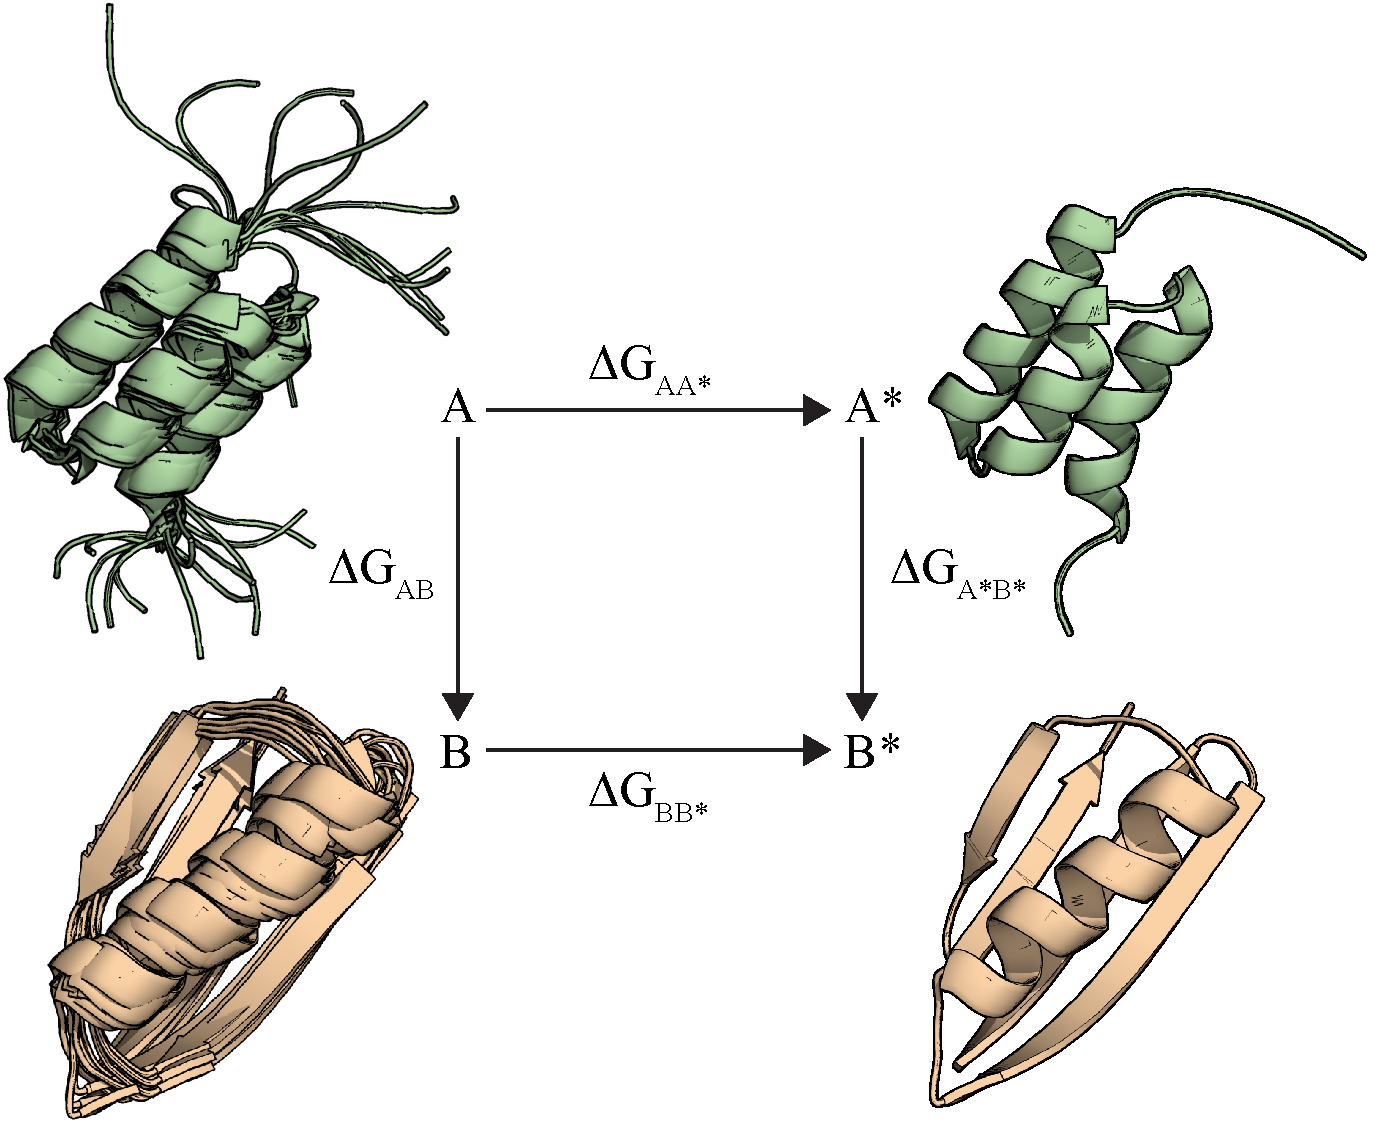
\includegraphics[width=14cm,height=14cm]{method.pdf}
\end{center}
\caption{Graphical representation of the thermodynamic cycle involving confinement method.}
\label{fig:method}
\end{figure}


\begin{figure} 
\begin{center} 
\includegraphics[width=12cm,height=10cm]{bhp.pdf}
\end{center}
\caption{Two conformations from $\beta$ hairpin from protein G, bhp1 and bhp2. The two stranded $\beta$ sheet, bhp1 is the native structure and the three stranded $\beta$ sheet is known as bhp3.}
\label{fig:bhp_conf}
\end{figure}

\begin{figure}
\begin{center}
\includegraphics[width=12cm,height=10cm]{G95.pdf}
\end{center}
\caption{Two protein with 95 \% similar sequence but different folds}
\label{fig:G95}
\end{figure}

\begin{figure}
\begin{center}
\includegraphics[width=12cm,height=10cm]{G88.pdf}
\end{center}
\caption{Two protein with 88 \% similar sequence but different folds}
\label{fig:G88}
\end{figure}

\begin{table}
\caption{The comparison of free energy values of proteins with 95 \% and 88 \% similar sequences in $3 \alpha$ and $4 \beta + \alpha$ fold.}
\label{tab:GA_GB}
\begin{center}
\begin{tabular}{l l l}\hline
Changes in   &     $\Delta G$ (Kcal/Mol) &  $\Delta G$ (Kcal/Mol) \\
 Sequences   &     ($3 \alpha$ fold)       & ($4 \beta + \alpha$ fold) \\ \hline
L20I30L45    &     $0.000$            &  $2.901 \pm 0.475$   \\
A20F30Y45    &     $4.365 \pm 0.460$ &  $0.000$    \\
G24I25I30I33 &     $0.000$            &  $ 3.941 \pm 0.517$ \\
L45I49L50    &                        &              \\
A24T25F30Y33 &     $5.576 \pm 0.464$  &  $0.000$     \\
Y45T49K50    &                        &             \\ \hline
\end{tabular}
\end{center}
\end{table}


\begin{figure}
\begin{center}
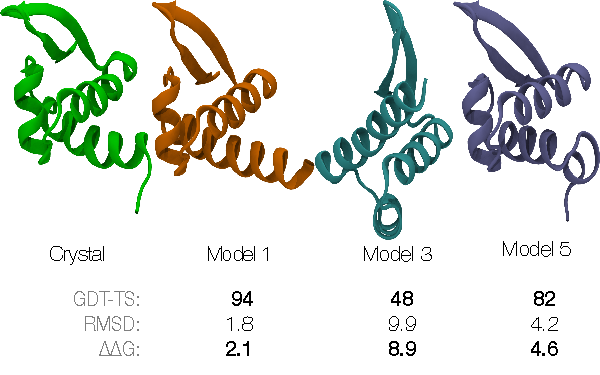
\includegraphics[width=12cm,height=10cm]{T0559.pdf}
\end{center}
\caption{Target T0559 from CASP9}
\label{fig:T0559}
\end{figure}

\begin{table}
\caption{The value of free energy and GDT\_TS for the CASP9 target T0559}
\label{tab:T0559}
\begin{center}
\begin{tabular}{l l l}\hline
Model   &     $\Delta G$ (Kcal/Mol) &  GDT\_TS \\ \hline
Model 1 &     0.000            &  94.03    \\
Model 3 &     $14.484 \pm 0.633$ &  48.13    \\         
Model 5 &     $4.526  \pm 0.384$ &  82.46    \\ \hline
\end{tabular}
\end{center}
\end{table}

\begin{figure}
\begin{center}
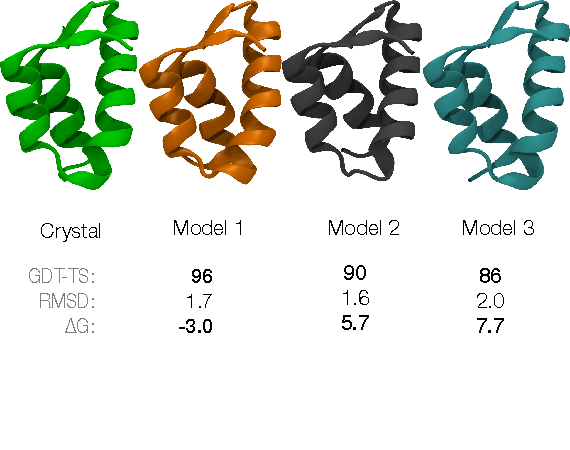
\includegraphics[width=12cm,height=10cm]{T0538.pdf}
\end{center}
\caption{Target T0538}
\label{fig:T0538}
\end{figure}

\begin{table}
\caption{The Free energy and GDT\_TS values of the CASP9 Target T0538}
\label{tab:T0538}
\begin{center}
\begin{tabular}{l l l l}\hline
Model   &     $\Delta G$ (Kcal/Mol) &  GDT\_TS & Group Submitted \\ \hline
Model 1 &     0.000              &  96.23    & PconsR  \\ 
Model 2 &     $15.891 \pm 0.475$ &  90.09  & Shell  \\ 
Model 3 &     $23.243 \pm 0.393$ &  86.32  & FOLDIT  \\ 
Model 4 &     $26.002 \pm 0.756$ &  80.66  & BAKER-ROSETTASERVER \\ \hline
\end{tabular}
\end{center}
\end{table}

\begin{figure}
\begin{center}
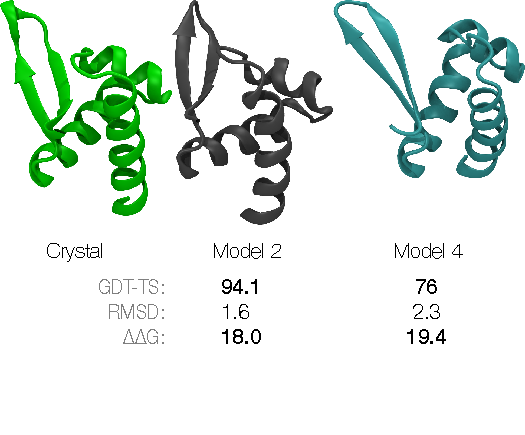
\includegraphics[width=12cm,height=10cm]{T0560.pdf}
\end{center}
\caption{Target T0560}
\label{fig:T0560}
\end{figure}

\begin{table}
\caption{The free energy and the GDT\_TS value of the CASP9 target T0560.}
\label{tab:T0560}
\begin{center}
\begin{tabular}{l l l}\hline
Model   &     $\Delta G$ (Kcal/Mol) &  GDT\_TS \\ \hline
Crystal &     0.000              & 100.00    \\
Model 2 &     $22.153 \pm 0.491$ &  94.14    \\
Model 4 &     $27.428  \pm 0.477$ &  76.56    \\ \hline
\end{tabular}
\end{center}
\end{table}


\begin{figure}
\begin{center}
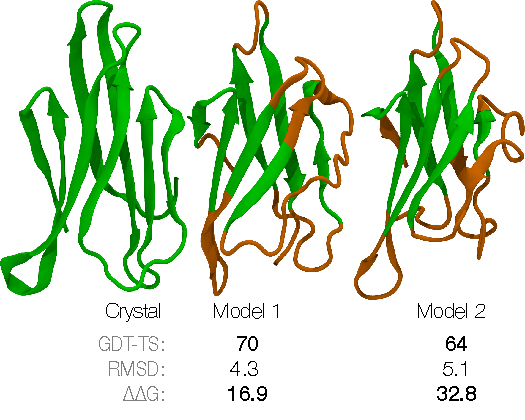
\includegraphics[width=12cm,height=10cm]{T0540.pdf}
\end{center}
\caption{T0540}
\label{fig:}
\end{figure}

\begin{table}
\caption{The free energy and the GDT\_TS value of the CASP9 target T0540.}
\label{tab:T0540}
\begin{center}
\begin{tabular}{l l l l}\hline
Model   &     $\Delta G$ (Kcal/Mol) &  GDT\_TS & Group Submitted \\ \hline
Crystal &     0.000              &  100.00   & -      \\ 
Model 1 &     $22.003 \pm 0.575$ &  69.72    & LTB    \\
Model 2 &     $53.786 \pm 0.553$ &  63.89    & Mufold \\ \hline
\end{tabular}
\end{center}
\end{table}

\begin{figure}
\begin{center}
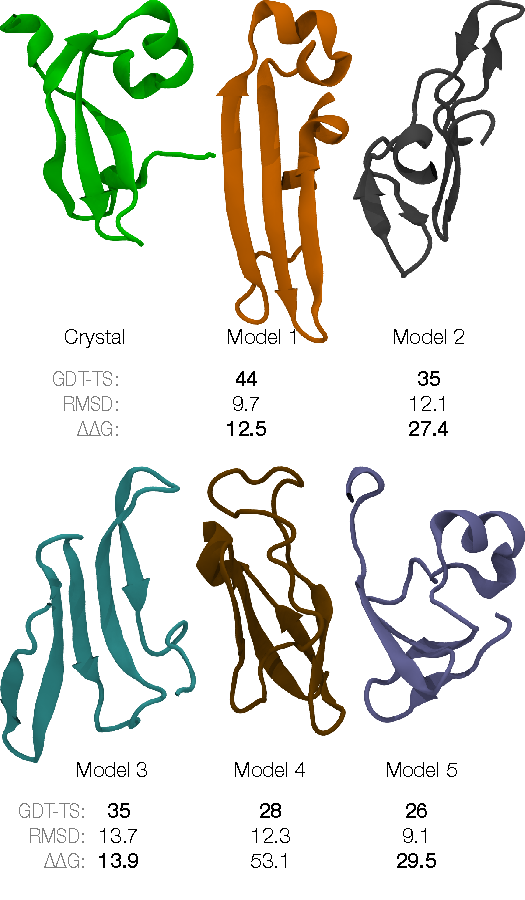
\includegraphics[width=12cm,height=10cm]{T0531.pdf}
\end{center}
\caption{T0531}
\label{fig:T0531}
\end{figure}

\begin{table}
\caption{The free energy and the GDT\_TS value of the CASP9 target T0531.}
\label{tab:T0531}
\begin{center}
\begin{tabular}{l l l}\hline
Model   &     $\Delta G$ (Kcal/Mol) &  GDT\_TS \\ \hline
Crystal &     0.000              & 100.00    \\
Model 1 &     $12.496 \pm 0.704$ &  43.53    \\
Model 2 &     $27.374 \pm 0.691$ &  34.48    \\
Model 3 &     $13.914 \pm 0.673$ &  34.48    \\
Model 4 &     $53.055 \pm 0.684$ &  28.02    \\
Model 5 &     $29.508 \pm 0.698$ &  25.86   \\ \hline
\end{tabular}
\end{center}
\end{table}

\begin{figure}
\begin{center}
\includegraphics[width=12cm,height=10cm]{T0605.pdf}
\end{center}
\caption{T0605}
\label{fig:T0605}
\end{figure}


\begin{table}
\caption{The free energy and the GDT\_TS value of the CASP9 target T0605.}
\label{tab:T0605}
\begin{center}
\begin{tabular}{l l l}\hline
Model   &     $\Delta G$ (Kcal/Mol) &  GDT\_TS \\ \hline
Model 1 &     $0.000$ &  $97.96$    \\
Model 2 &     $1.689 \pm ?$ &  $89.29$    \\
Model 5 &     $16.064 \pm ?$ & $93.88$   \\ \hline
\end{tabular}
\end{center}
\end{table}



\section{Conclusion}



\bibliographystyle{achemso}
\bibliography{paper}

Ytreberg, F.; Zuckerman, D. Simple estimation of absolute free energies for biomolecules. J. Chem. Phys. 2006, 124, 104105.

Park, S.; Lau, A.; Roux, B. Computing conformational free energy by deactivated morphing. J. Chem. Phys. 2008, 129, 134102

Zheng, L.; Chen, M.; Yang, W. Random walk in orthogonal space to achieve efficient free-energy simulation of complex systems, Proc. Natl. Acad. Sci. 2008, 105 (51), 20227.

Tyka, M.; Clarke, A.; Sessions, R. An Efficient, Path-Independent Method for Free-Energy Calculations. J.Phys.Chem. B 2006, 110, 17212–17220.


\end{document}

